\begin{minipage}{\linewidth}
\begin{center}

\begin{minipage}{\linewidth}
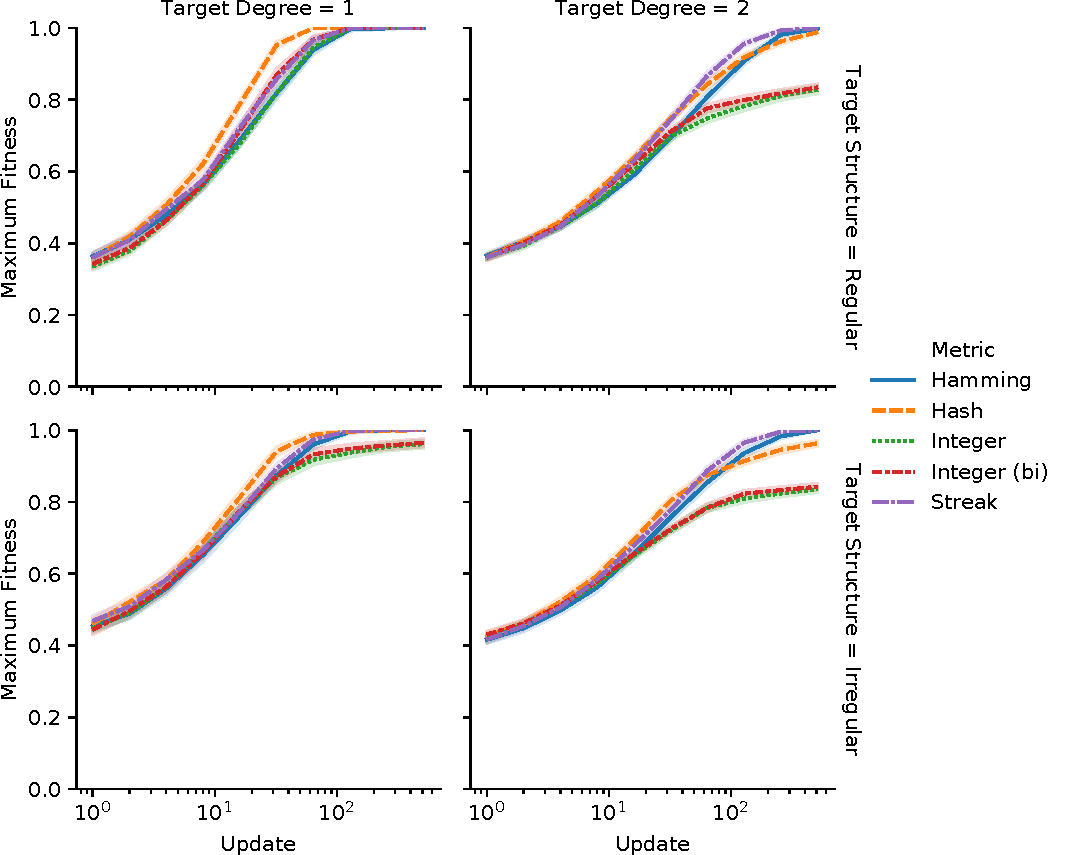
\includegraphics[width=\linewidth]{target_evolve/viz=max-fitness-line+_data_hathash_hash=673d309ab90e91d1+_script_fullcat_hash=fe3ddc711c5abfad+ext=}
\end{minipage}
\begin{minipage}{\linewidth}
\caption{
Maximum fitness by update over replicate runs for each metric's best-performing mutation rate.
Note log-scale x-axes.
Shaded area represents 95\% confidence intervals.
}
\label{fig:evolve_bests}
\end{minipage}
\end{center}
\end{minipage}


\begin{figure}[]{\linewidth}
\centering
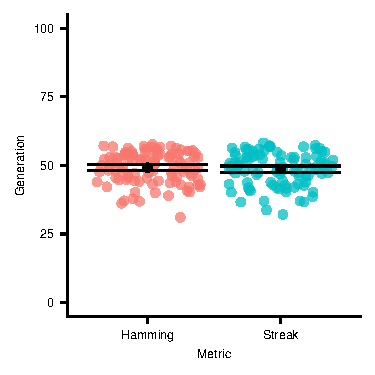
\includegraphics[width=\linewidth]{img/gp_results/panel-cst-times.pdf}%
\caption{
 CST TODO
 }
\label{fig:cst-times}
\end{figure}


\begin{figure*}
\begin{minipage}{6in}
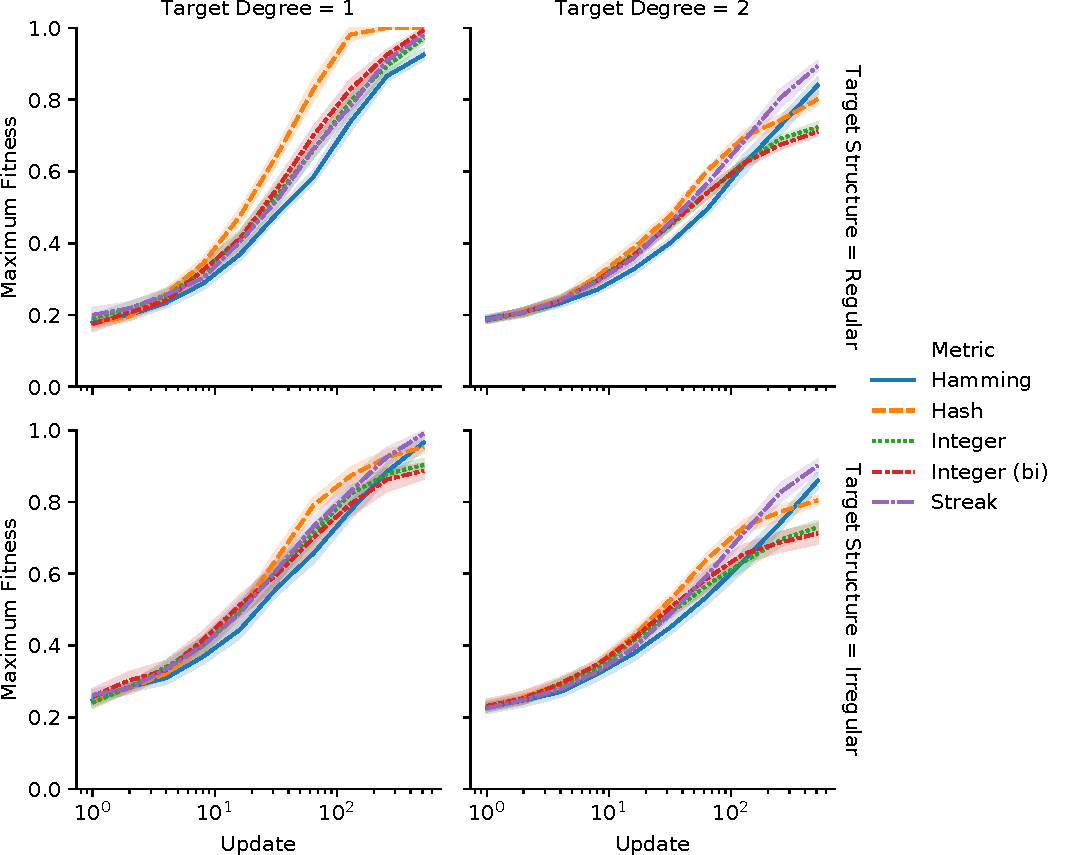
\includegraphics[width=\textwidth]{img/target_evolve_big/viz=max-fitness-line+_data_hathash_hash=4db1200f9d71a980+_script_fullcat_hash=fe3ddc711c5abfad+ext=}
\caption{64-node target graph}
\label{fig:evolve_big_bests}
\end{minipage}
\begin{minipage}{\textwidth}
\caption{
Trajectories of adaptive evolution for each tag-matching metric on the 64-node graph-matching task.
Maximum fitness represents the best fitness value for any individual within a population.
Here report using each metric's best-performing per-bit mutation rate.
(See Supplementary Figure \ref{fig:evolve_big_mutsweep} for survey showing how mutation rate affects adaptive evolution under each metric.)
Note log-scale x-axes.
Shaded area represents bootstrapped 95\% confidence intervals across 20 replicate observations.
}
\label{fig:evolve_bests64}
\end{minipage}
\end{figure*}


\begin{figure*}
\begin{center}

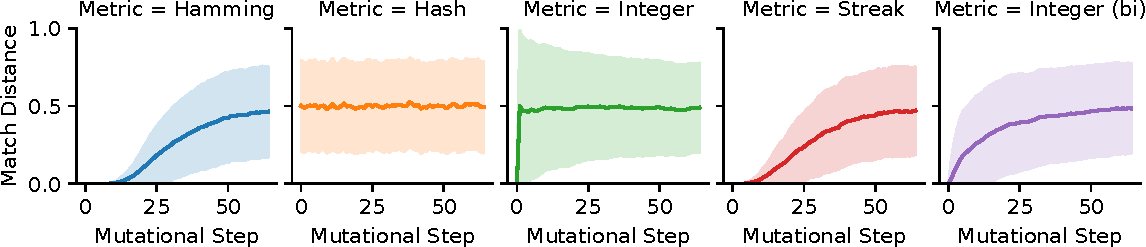
\includegraphics[width=\textwidth]{{{mutational_walk/bitweight=0.5+seed=1+title=mutational_walk_lineplot+_data_hathash_hash=ff15c8831d4f9288+_script_fullcat_hash=c872df869f05035a+ext=}}}
\caption{
TODO
}
\label{fig:mutational_walk_lineplot}

\end{center}
\end{figure*}


\begin{figure}[!htbp]
\begin{center}

\begin{subfigure}{\textwidth}
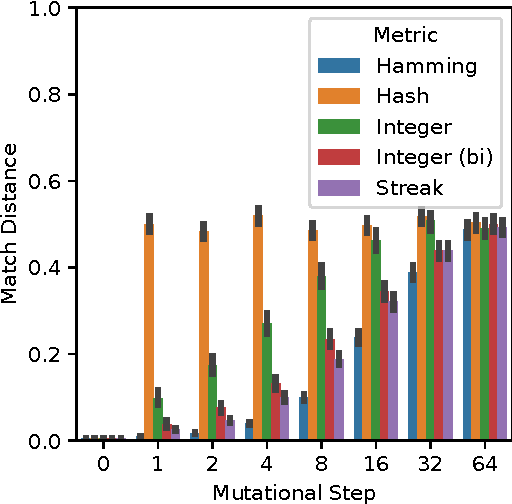
\includegraphics[width=\textwidth]{img/mutational_walk_sampled_start/bitweight=0dot5+seed=1+title=mutational_walk_barplot+_data_hathash_hash=05b961e08b5b7854+_script_fullcat_hash=982405ca713eba73+ext=}
\caption{
Error bars represent 95\% confidence intervals.
Note logarithmic scale on the $x$ axis.
}
\label{fig:mutational_walk_sampled_start_barplot}
\end{subfigure}

\begin{subfigure}{\textwidth}
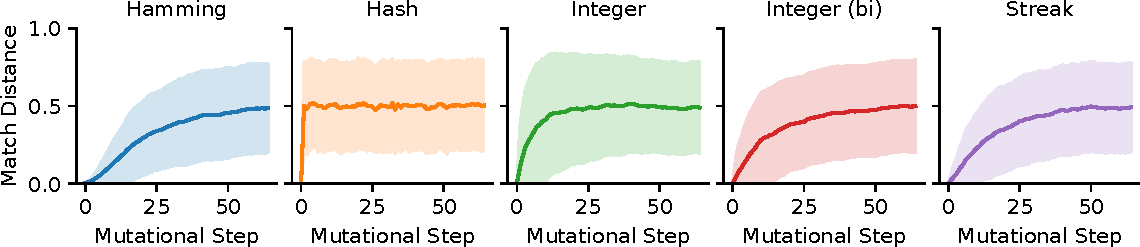
\includegraphics[width=\textwidth]{img/mutational_walk_sampled_start/bitweight=0dot5+seed=1+title=mutational_walk_lineplot+_data_hathash_hash=05b961e08b5b7854+_script_fullcat_hash=982405ca713eba73+ext=.pdf}
\caption{
Alternate visualization, shaded area represents standard deviation.
}
\end{subfigure}

\caption{
Match distance along mutational walks from 32-bit tags sampled for initial match distance $<0.01$.
}
\label{fig:mutational_walk_sampled_start}

\end{center}
\end{figure}


\begin{figure}
\begin{center}

\begin{subfigure}{\textwidth}
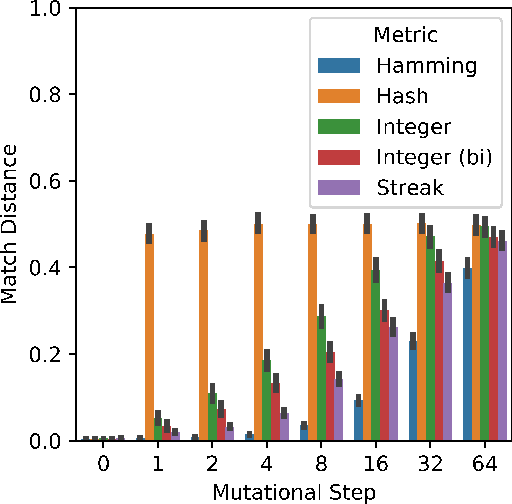
\includegraphics[width=\textwidth]{img/mutational_walk_sampled_start_64/bitweight=0dot5+seed=1+title=mutational_walk_barplot+_data_hathash_hash=2137b5ab8659c35e+_script_fullcat_hash=982405ca713eba73+ext=}
\caption{
Error bars represent 95\% confidence intervals.
Note logarithmic scale on the $x$ axis.
}
\label{fig:mutational_walk_sampled_start_64_barplot}
\end{subfigure}

\begin{subfigure}{\textwidth}
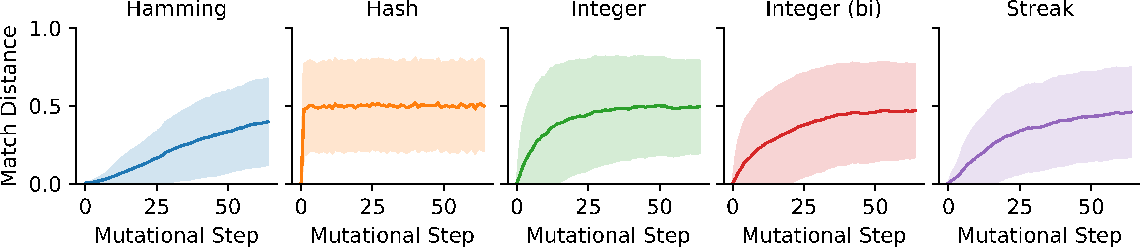
\includegraphics[width=\textwidth]{img/mutational_walk_sampled_start_64/bitweight=0dot5+seed=1+title=mutational_walk_lineplot+_data_hathash_hash=2137b5ab8659c35e+_script_fullcat_hash=982405ca713eba73+ext=}
\caption{
Alternate visualization, shaded area represents standard deviation.
}
\end{subfigure}

\caption{
Match distance along mutational walks from 64-bit tags sampled for initial match distance $<0.01$.
}
\label{fig:mutational_walk_sampled_start}

\end{center}
\end{figure}


\begin{figure*}[!htbp]
\begin{minipage}{6in}
\begin{center}

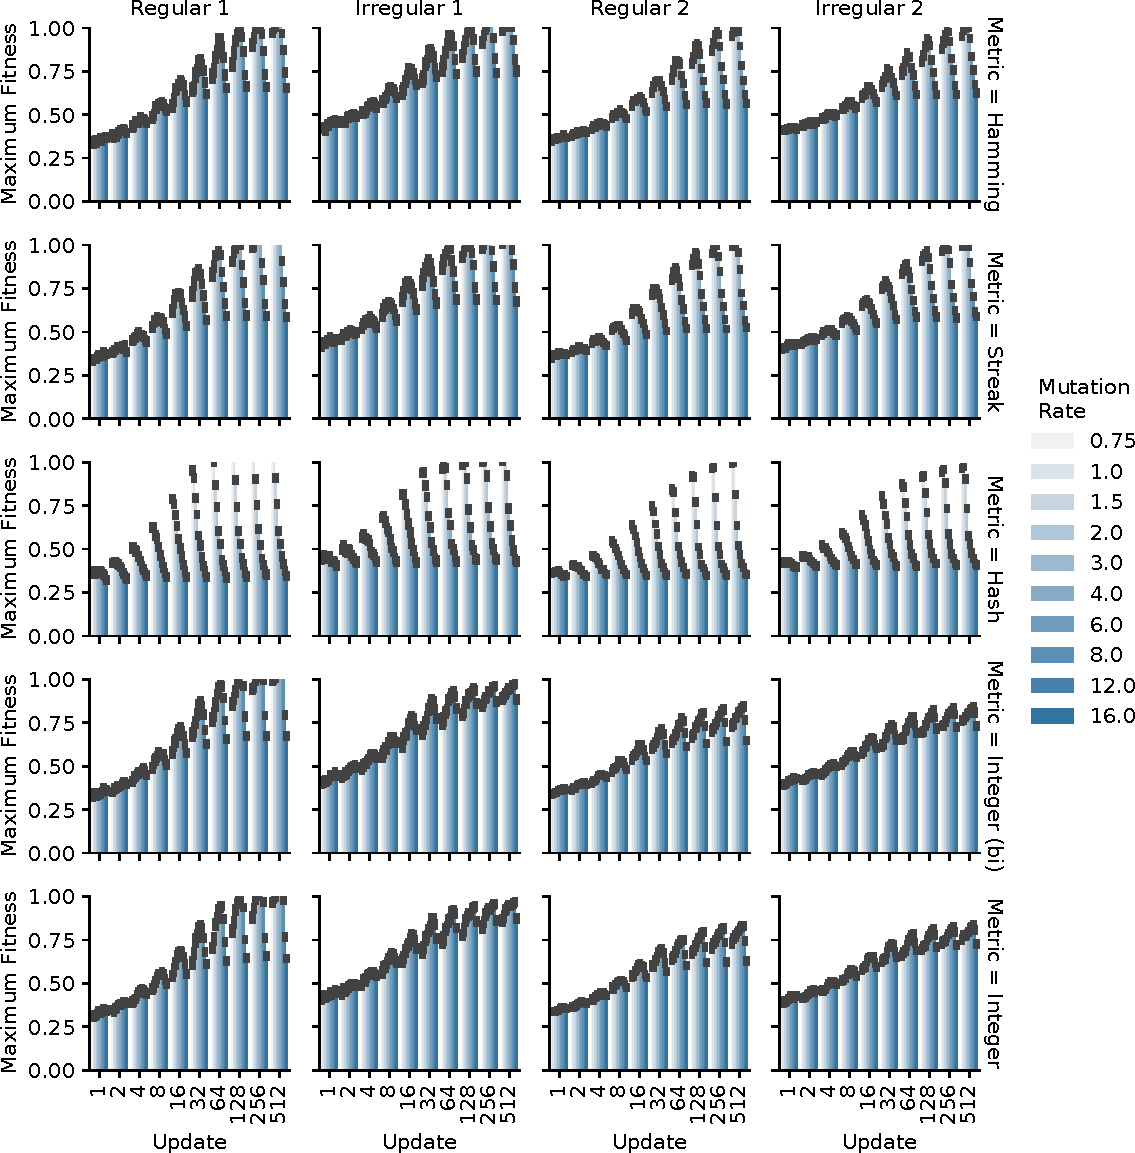
\includegraphics[width=\textwidth]{img/target_evolve/title=fitness_mutation_barplot+_data_hathash_hash=4c78832f20b46ffd+_script_fullcat_hash=6ccad43c80699be8+ext=}
\caption{
32-node graph-matching task mutation rate sensitivity analysis.
Metrics exhibited fastest adaptive evolution within the range of mutation rates surveyed, except the hash metric which exhibited fastest adaptive evolution at at the lowest mutation rate surveyed.
Maximum fitness is the best fitness value for any individual within a population.
Maximum fitness at each update is presented across the range of surveyed mutation rates.
Error bars represent bootstrap 95\% confidence intervals across 50 replicate populations.
}
\label{fig:evolve_mutsweep}

\end{center}
\end{minipage}
\end{figure*}


\begin{figure*}
\begin{center}

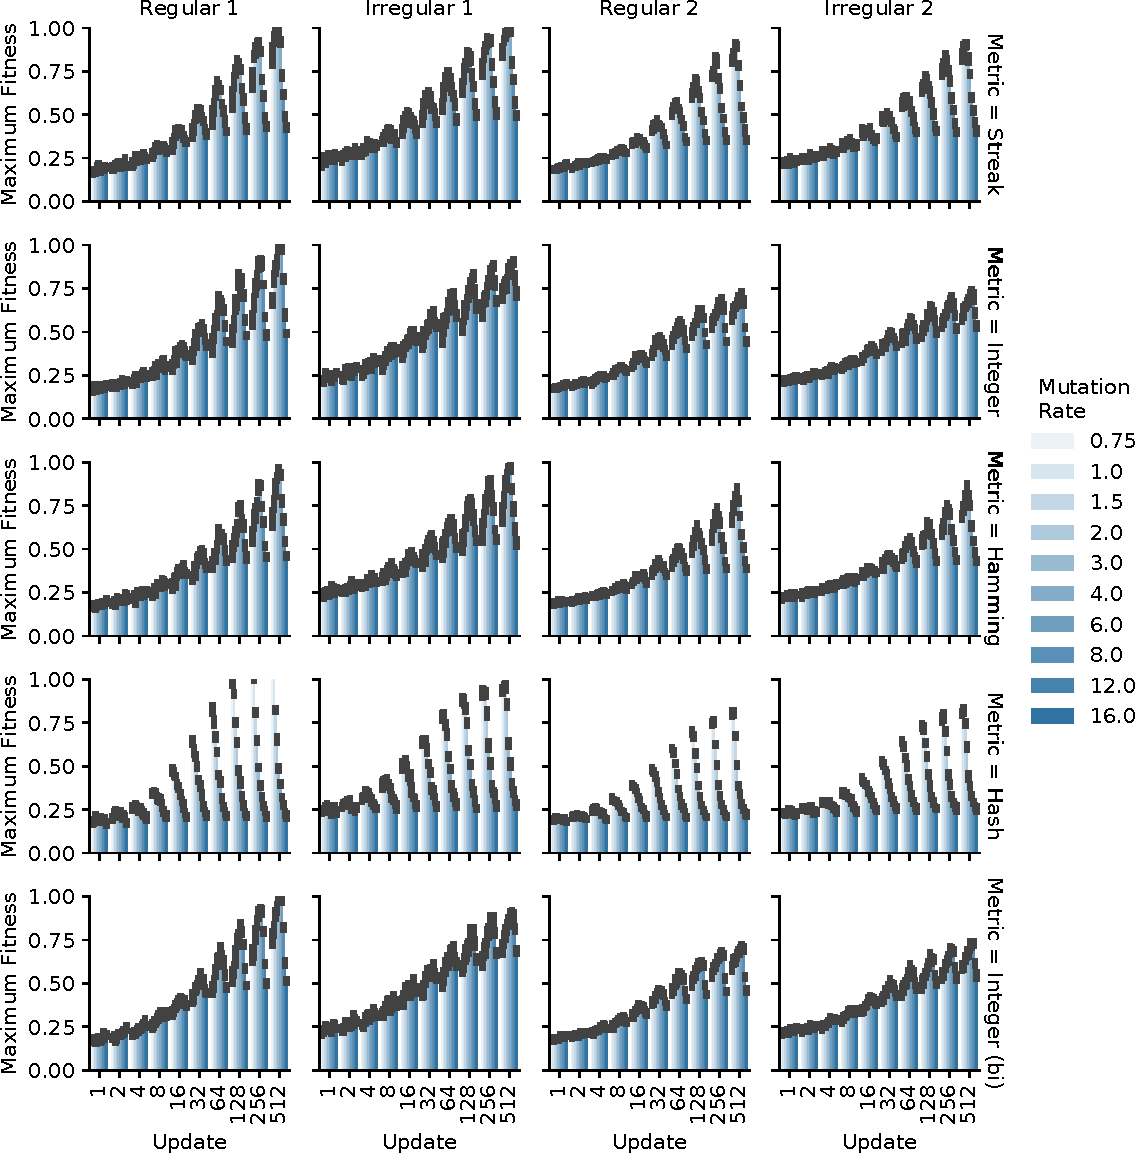
\includegraphics[width=\textwidth]{target_evolve_big/title=fitness_mutation_barplot+_data_hathash_hash=4db1200f9d71a980+_script_fullcat_hash=fe3ddc711c5abfad+ext=}
\caption{
Maximum fitness among replicate runs across a set of per-bit mutation rates.
Error bars represent 95\% confidence intervals.
}
\label{fig:evolve_mutsweep}

\end{center}
\end{figure*}


\section{Hamming Metric} \label{sec:hammingmetric}

Each tag was represented as an ordered, fixed-length bitstring,
\begin{align*}
t = \langle t_0, t_1, t_2, \dots, t_{n-2}, t_{n-1} \rangle
\end{align*}
where
\begin{align*}
\forall i, t_i \in \{0, 1\}.
\end{align*}

This metric is based on the work of \citep{lalejini2019else}, originally after TODO hamming cite(?).

In this metric, we compare tags according to their bitwise hamming distance.
Mathematically speaking for tags $t$ and $u$ we compute the distance according to the metric $M$ as,
\begin{align*}
M(t, u)
= \frac{
  \#\{ i : t_i \neq u_i, i=0, \dots ,n-1\}
}{
  n
}
\end{align*}

This metric is commutative and $n$-dimensional.




\section{Hash Metric} \label{sec:hashmetric}

This metric is original to the our paper and meant to serve as a control.

The an arbitrary, but determinsitic value, uniformly distributed between 0 and 1.

We rely on the \texttt{hash\_combine} function, adapted from BOOST (TODO cite).

for two values \texttt{v1} and \texttt{v2}, \texttt{hash\_combine} is defined as follows
\begin{verbatim}
unsigned int hash_combine(
  unsigned int v1,
  unsigned int v2
) {
  return v1 ^ (
    v2 * 0x9e3779b9
    + (v1 << 6) + (v1 >> 2)
  );
}
\end{verbatim}

We compute the hash value of a tag as follows
\begin{verbatim}
unsigned int h(unsigned char *tag) {
  unsigned int result = tag[0];
  for (int i = 1; i < 4; ++i){
    result = hash_combine(result, t[i]);
  }
  return result;
}
\end{verbatim}
where \texttt{tag} is the tag's bitstring stored as an array of bytes.

To compute the metric $H$ we then call \texttt{hash\_combine} to combine the hash values of the tags $t$ and $u$
\begin{align*}
H(t, u) = \texttt{hash\_combine( h(}t\texttt{), h(}u\texttt{))}
\end{align*}

Note that this is not commutative.




\section{Integer Metric}
\label{sec:integermetric}

Each tag was represented as an ordered, fixed-length bitstring,
\begin{align*}
t = \langle t_0, t_1, t_2, \dots, t_{n-2}, t_{n-1} \rangle
\end{align*}
where
\begin{align*}
\forall i, t_i \in \{0, 1\}.
\end{align*}

This metric is inspired by \citep{spector2011tag}.
They used positive integers between 0 and 100 to name referents.
Queries were provided the referent that had the next-larger value, wrapping around from 100 back to 0.

In this metric, we compare tags according to their value as an unsigned integer according to the following representation $f$,
\begin{align*}
f(t)
= \sum_{i=0}^{n-1} t_i \times 2^i.
\end{align*}

The distance metric $I$ between two length-$n$ tags $t$ and $u$ is
\begin{align*}
I(t, u) =
\begin{cases}
  \frac{2^n - f(t) + f(u)}{2^n}, & \text{if } f(t) > f(u), \\
  \frac{f(t) - f(u)}{2^n},         & \text{else} f(t) \leq f(u).
\end{cases}
\end{align*}

Note that this metric is non-commutative, i.e., it is not necessarily true that $I(t, u) = I(u, t)$.

Note also that this metric is one-dimensional.

A algorithmic advantage of this metric is that it allows for log-time matching.




\subsection{Bidirectional Integer Metric} \label{sec:integerbimetric}

Each tag was represented as an ordered, fixed-length bitstring,
\begin{align*}
t = \langle t_0, t_1, t_2, \dots, t_{n-2}, t_{n-1} \rangle
\end{align*}
where
\begin{align*}
\forall i, t_i \in \{0, 1\}.
\end{align*}

This metric is inspired by \citep{spector2011tag}.
They used positive integers between 0 and 100 to name referents.
Queries were provided the referent that had the next-larger value, wrapping around from 100 back to 0.

In this metric, we compare tags according to their value as an unsigned integer according to the following representation $f$,
\begin{align*}
f(t)
= \sum_{i=0}^{n-1} t_i \times 2^i.
\end{align*}

The distance metric $I$ between two length-$n$ tags $t$ and $u$ is
\begin{align*}
I(t, u) =
\begin{cases}
  \frac{2^n - f(t) + f(u)}{2^n}, & \text{if } f(t) > f(u), \\
  \frac{f(t) - f(u)}{2^n},         & \text{else} f(t) \leq f(u).
\end{cases}
\end{align*}

Note that this metric is non-commutative, i.e., it is not necessarily true that $I(t, u) = I(u, t)$.

Note also that this metric is one-dimensional.




\section{Streak Metric} \label{sec:streakmetric}

Each tag was represented as an ordered, fixed-length bitstring,
\begin{align*}
t = \langle t_0, t_1, t_2, \dots, t_{n-2}, t_{n-1} \rangle
\end{align*}
where
\begin{align*}
\forall i, t_i \in \{0, 1\}.
\end{align*}

This metric was originally proposed by \citep{downing2015intelligence}.
Downing claims that it exhibits
It is computed according to the ratio between the longest contiguously matching substring among two bitsets and the longest contiguously mismatching substring among those two bitsets.
Downing claims that this metric exhibits greater robustness compared to integer and hamming distance metrics using mutational walk experiments but does not demonstrate it in an evolving system.

We define the greatest contiguously-matching length of $n$-long bitstrings $t$ and $u$ as follows,
\begin{align*}
m(t, u) = \max(\{i - j \forall i, j \in 0..n-1 \mid \forall q \in i..j, t_q = u_q \})
\end{align*}

We define the greatest contiguously-mismatching length as follows,
\begin{align*}
n(t, u) = \max(\{i - j \forall i, j \in 0..n-1 \mid \forall q \in i..j, t_q \neq u_q \})
\end{align*}

The streak metric $S'$  with tags $t$ and $u$
\begin{align*}
S'(t, u)
= \frac{ p(n(t,u)) }{p(m(t,u)) + p(n(t,u))}.
\end{align*}
where $p$ approximates the probability of a contiguously-matching substring between

It is worth noting that the formula for computing the probability of a $k$-bit match or mismatch, given by Downing as follows, is actually mathematically flawed.
\begin{align*}
p_k
= \frac{n - k + 1}{2^k}
\end{align*}

The probability of a $0$-bit match according to this formula would be computed as $p_0 = \frac{n - 0 + 1}{2^0} = n + 1$ which is clearly impossible because $p_0 > 1 \forall n > 0$.
The actual can probability be achieved using a lookup table computed using dynamic programming.

However, the formula Downing presented provides a useful approximation to the probability of a $k$ bit match.
For computational efficiency and consistency with the existing literature we use clamp edge cases between 0 and 1 to yield the corrected streak metric $S$.

\begin{align*}
S(t, u) =
\max( \min( S'(t, u), 1), 0)
\end{align*}




\section{Detour Difference}

\begin{figure}
\begin{center}

\begin{minipage}{\linewidth}
\begin{subfigure}[b]{\linewidth}
\begin{minipage}{0.5\textwidth}
\begin{center}
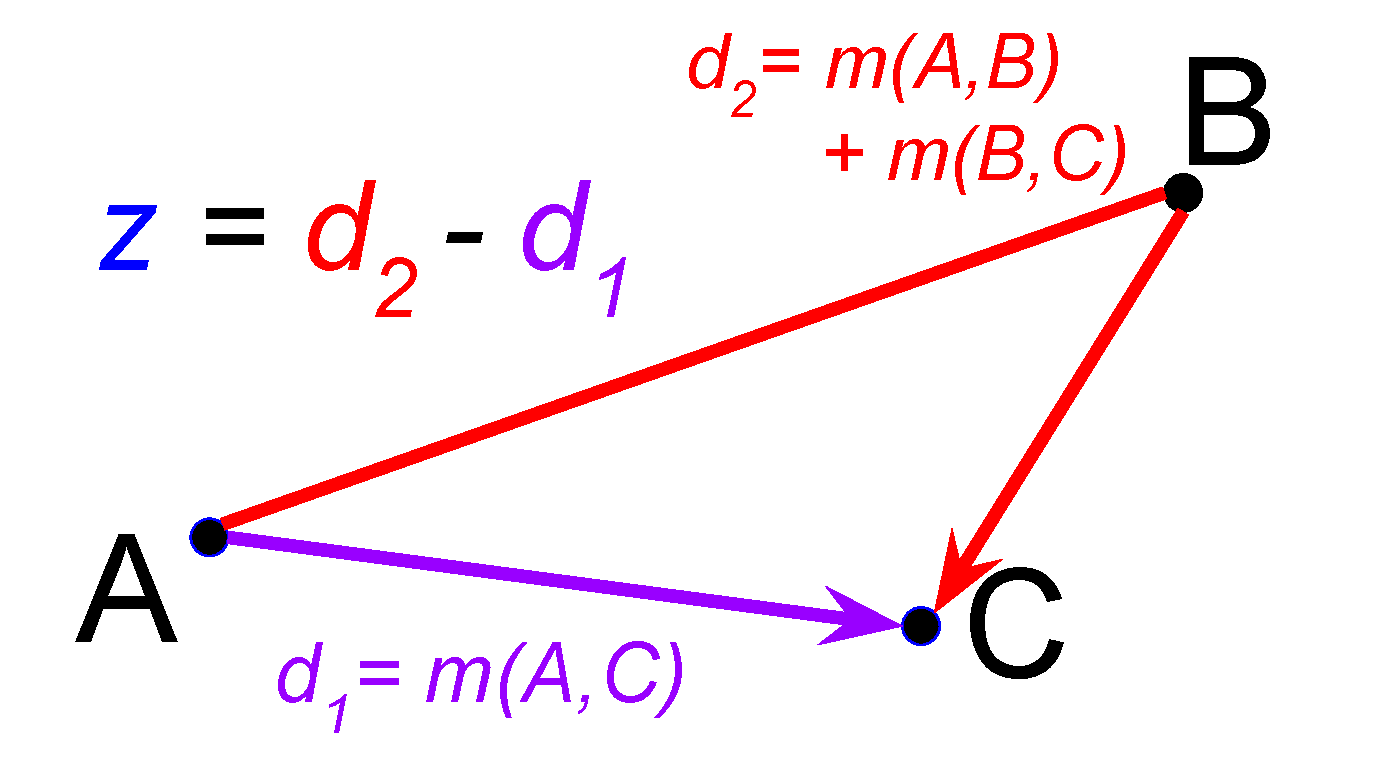
\includegraphics[width=\linewidth,trim=2cm 5cm 2cm 5cm, clip]{detour-difference}
\end{center}
\end{minipage}%
\begin{minipage}{0.5\textwidth}
\caption{
Sampling process used to evaluate detour difference, $z$.
} \label{fig:detour_difference_cartoon}
\end{minipage}
\end{subfigure}
\end{minipage}

\begin{minipage}{\linewidth}
\begin{subfigure}[b]{\linewidth}
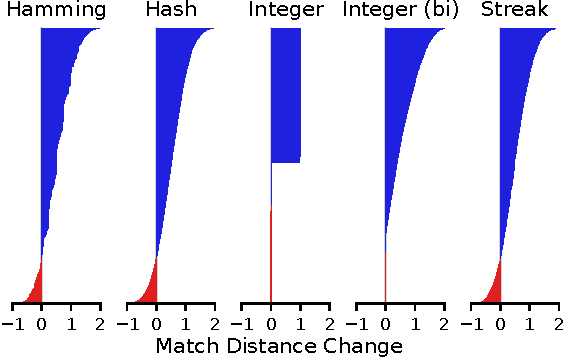
\includegraphics[width=\linewidth]{detour_difference/bitweight=0dot5+seed=1+title=low-triplet-analysis+_data_hathash_hash=6b0749ef97a58721+_script_fullcat_hash=297c4fe09078e17b+ext=}
\caption{
Distributions of detour distance difference for triplets of randomly sampled tags.
Each bar sliver represents an independently sampled observation.
A positive value (colored blue) indicates that total distance increased with the addition of an intermediate stop.
A value of exactly 0 indicates an intermediate stop had no effect on total distance.
A negative value (colored red) indicates violation of the triangle inequality: taking an intermediate stop reduced the total distance travelled.
} \label{fig:detour_difference_distribution}

\end{subfigure}
\end{minipage}

\caption{
Detour difference of tag-matching metrics.
}
\label{fig:detour_difference}

\end{center}
\end{figure}


To get a sense of the regularity, in a looses sense, of each space we uniformly sampled triplets of points $A$, $B$, and $C$.
Then, for each metric $m$ we calculated the statistic $m(A, B) + m(B, C) - m(A, C)$.
If the triangle inequality is respected this statistic should be greater than or equal to zero.
Figure \ref{fig:detour_difference} plots the distribution of this statistic for each metric.
The hamming, hash, and streak metrics show evidence of ``shortcuts'' that violate the triangle inequality.
It should be noted that the raw hamming metric does respect the triangle inequality.





To get a sense of the regularity, in a looses sense, of each space we uniformly sampled triplets of points $A$, $B$, and $C$.
Then, for each metric $m$ we calculated the statistic $m(A, B) + m(B, C) - m(A, C)$.
If the triangle inequality is respected this statistic should be greater than or equal to zero.
Figure \ref{fig:detour_difference} plots the distribution of this statistic for each metric.
The hamming, hash, and streak metrics show evidence of ``shortcuts'' that violate the triangle inequality.
It should be noted that the raw hamming metric does respect the triangle inequality.

\section{Genetic Programming Experiments}
\label{sec:gpsupplement}


\subsection{SignalGP}

SignalGP (Signal-driven Genetic Programs) is a GP representation that enables signal-driven (\textit{i.e.}, event-driven) program execution.
In SignalGP, programs are segmented into modules (functions) that may be automatically triggered by exogenously- or endogenously-generated signals.
Each module in SignalGP associates a tag with a linear sequence of instructions.
SignalGP makes explicit the concept of signals (events), which comprise a tag and, optionally, signal-specific data.
Signals trigger the module with the closest matching tag (according to a given tag-matching scheme), using any signal-associated data as input to the triggered module.
SignalGP can handle many signals simultaneously, processing each in parallel.

The SignalGP instruction set, in addition to including traditional GP operations, allows programs to generate internal signals, broadcast external signals, and otherwise work in a tag-based context.
Instructions contain arguments, including an evolvable tag, that may modify the instruction's effect, often specifying memory locations or fixed values.
Instructions may refer to program modules using tag-based referencing; for example, an instruction may trigger the execution of a program module using the instruction's tag to specify which module to trigger.
SignalGP also supports genetic regulation with promoter and repressor instructions that, when executed, allow programs to adjust how well subsequent signals match with a target function (specified with tag-based referencing).

See \citepinappendix{lalejini2018evolving} for a more detailed description of the SignalGP representation. Additionally, see the GitHub repository for the SignalGP implementation used in this work \citepinappendix{lalejini_2020_3781295}.

\subsection{Changing-signal Task Description}

The changing-signal task requires programs to express a distinct response to each of $K$ environmental signal (each signal has a unique tag).
Programs express a response by executing one of $K$ response instructions.
Successful programs can `hardcode' each response with the appropriate environmental signal, ensuring that each environmental signal's tag best matches the function containing the correct response.
We expect the particular metric used to match tags to influence how well programs adapt to changing-signal task.

During evaluation, we afford programs 64 time steps to express the appropriate response after receiving a signal.
Once a program expresses a response or the allotted time expires, we reset the program's virtual hardware (resetting all executing threads and thread-local memory), and the environment produces the next signal.
Evaluation continues until the program correctly responds to each of the $K$ environmental signals or until the program expresses an incorrect response.
During each evaluation, programs experience environmental signals in a random order; thus, the correct \textit{order} of responses will vary and cannot be hardcoded.

% Experiment overview
For each metric, we evolved 200 replicate populations (each with a unique random number seed) of 500 asexually reproducing programs in an eight-signal environment ($K=8$) for 100 generations.
We identified the most performant tag mutation rate (from a range of possible mutation rates) for each metric to use in our experiment.
These data (and analyses) are available online in the GitHub repository that houses these experiments \citepinappendix{lalejini_2020_3781295}.
We used the following per-bit tag mutation rates for the changing-signal task: 0.01 for the Hamming and Streak metrics, 0.002 for the Hash metric, and 0.02 for the Integer and Bidirectional Integer metrics.
Aside from tag mutation rate, the overall configuration used for each metric was identical.
We limited tag variation in offspring to tag mutation operators (bit flips) by initializing populations with a common ancestor program in which all tags are identical and by disallowing mutations that would insert instructions with random tags.

The full configuration details for the changing-signal task (including a guide to running these experiments on your local machine) can be found in the associated GitHub repository \citepinappendix{lalejini_2020_3781295}.

\subsection{Directional-signal Task Description}

% Task overview
As in the changing-signal task, the directional-signal task requires that programs respond to a sequence of environmental cues; in the directional-signal task, however, the correct response depends on previously experienced signals.
In the directional signal task, there are two possible environmental signals --- a `forward-signal' and a `backward-signal' (each with a distinct tag) ---  and four possible responses.
If a program receives a forward-signal, it should express the next response, and if the program receives, a backward-signal, it should express the previous response.
For example, if response-three is currently required, then a subsequent forward-signal indicates that response-four is required next, while a backward-signal would instead indicate that response-two is required next.
Because the appropriate response to both the backward- and forward-signals change over time, successful programs must regulate which functions these signals trigger (rather than hardcode each response to a particular signal).

% Evaluation overview
We evaluate programs on all possible four-signal sequences of forward- and backward-signals (sixteen total).
For each program, we evaluate each sequence of signals independently, and a program's fitness is equal to its aggregate performance.
Otherwise, evaluation on a single sequence of signals mirrors that of the changing signal task.

% Experiment overview
We used an identical experimental design for the directional-signal task as in the changing-signal task. 
However, we evolved programs for 5000 generations (instead of 100) and re-parameterized each metric's tag mutation rate (these data are available in the associated GitHub repository \citepinappendix{lalejini_2020_3781295}): 
0.001 for the Hamming and Hash metrics, 0.002 for the Integer and Streak metrics, and 0.0001 for the Bidirectional Integer Metric. 

The full configuration details for the directional-signal task (including a guide to running these experiments on your local machine) can be found in the associated GitHub repository \citepinappendix{lalejini_2020_3781295}.

\subsection{Data analysis and Implementation}

The source code for our GP experiments can be found in the following GitHub repository: \citepinappendix{lalejini_2020_3781295}. This repository additionally includes all data analysis and visualization scripts, experiment configuration details, and a guide for running our experiments locally.



